\documentclass[tikz,border=3pt]{standalone}
\usepackage[utf8]{inputenc}
\usepackage[T1]{fontenc}
\usepackage{lmodern}
\renewcommand{\familydefault}{\sfdefault}
\usepackage{sansmath}\sansmath
\usepackage{chemfig}
\usepackage{pgfplots}\pgfplotsset{compat=1.18,/pgf/number format/use comma,/pgf/number format/1000 sep={.}}
\usetikzlibrary{arrows.meta,calc,positioning,decorations.pathmorphing,patterns}
% paleta del sitio
\definecolor{nar}{HTML}{E8680C}\definecolor{narc}{HTML}{FFB35C}\definecolor{hielo}{HTML}{FFF3E8}
\definecolor{tinta}{HTML}{1D1D1F}\definecolor{gris}{HTML}{6E6E73}\definecolor{lila}{HTML}{7C5CF0}
\definecolor{azul}{HTML}{2F6FD6}\definecolor{menta}{HTML}{17A673}\definecolor{coral}{HTML}{E8342A}
\tikzset{na/.style={circle,draw=coral,fill=coral!15,inner sep=0.6pt,font=\scriptsize,text=coral,minimum size=0.62cm},
         k/.style={circle,draw=azul,fill=azul!15,inner sep=0.6pt,font=\scriptsize,text=azul,minimum size=0.62cm}}
\begin{document}
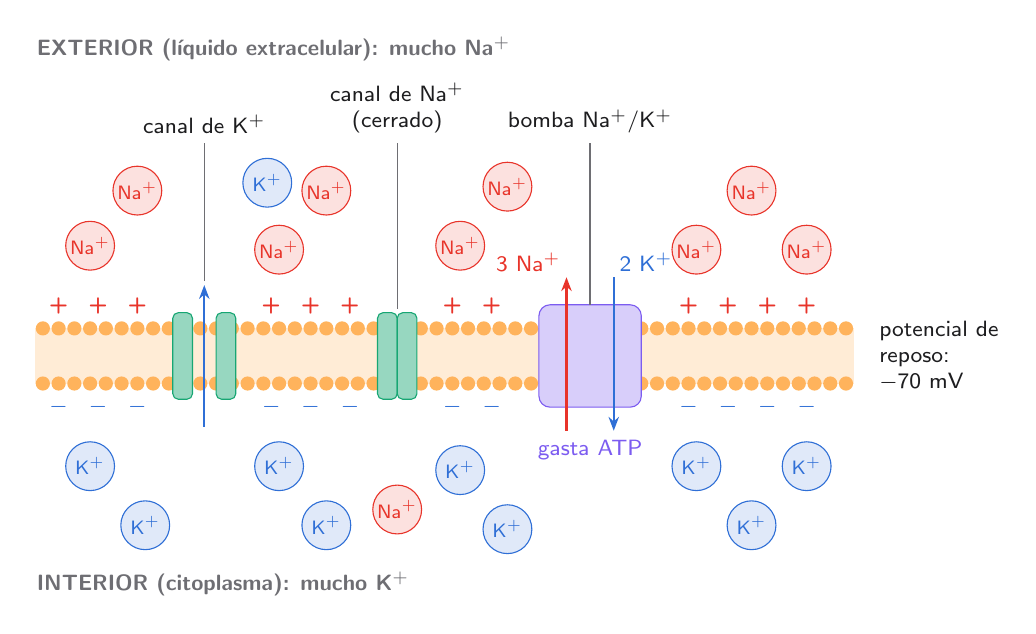
\begin{tikzpicture}[font=\small]
% membrana
\fill[narc!25] (0,0) rectangle (10.4,0.7);
\foreach \x in {0.1,0.3,...,10.3}{\fill[narc] (\x,0.7) circle (0.09); \fill[narc] (\x,0) circle (0.09);}
% canal de K+ (abierto)
\fill[menta!45,draw=menta,rounded corners=2pt] (1.75,-0.2) rectangle (2.0,0.9);
\fill[menta!45,draw=menta,rounded corners=2pt] (2.3,-0.2) rectangle (2.55,0.9);
\draw[-{Stealth[length=5pt]},azul,thick] (2.15,-0.55) -- (2.15,1.25);
% canal de Na+ (cerrado)
\fill[menta!45,draw=menta,rounded corners=2pt] (4.35,-0.2) rectangle (4.6,0.9);
\fill[menta!45,draw=menta,rounded corners=2pt] (4.6,-0.2) rectangle (4.85,0.9);
% bomba
\fill[lila!30,draw=lila,rounded corners=4pt] (6.4,-0.3) rectangle (7.7,1.0);
\draw[-{Stealth[length=5pt]},coral,thick] (6.75,-0.6) -- (6.75,1.35);
\draw[-{Stealth[length=5pt]},azul,thick] (7.35,1.35) -- (7.35,-0.6);
\node[coral,font=\footnotesize,anchor=south east] at (6.8,1.3) {3 Na$^+$};
\node[azul,font=\footnotesize,anchor=south west] at (7.3,1.3) {2 K$^+$};
\node[lila,font=\footnotesize] at (7.05,-0.85) {gasta ATP};
% cargas
\foreach \x in {0.3,0.8,1.3,3.0,3.5,4.0,5.3,5.8,8.3,8.8,9.3,9.8}{\node[coral,font=\footnotesize\bfseries] at (\x,0.98) {+};}
\foreach \x in {0.3,0.8,1.3,3.0,3.5,4.0,5.3,5.8,8.3,8.8,9.3,9.8}{\node[azul,font=\footnotesize\bfseries] at (\x,-0.3) {$-$};}
% iones exterior
\foreach \p in {(0.7,1.75),(1.3,2.45),(3.1,1.7),(3.7,2.45),(5.4,1.75),(6.0,2.5),(8.4,1.7),(9.1,2.45),(9.8,1.7)}{\node[na] at \p {Na$^+$};}
\node[k] at (2.95,2.55) {K$^+$};
% iones interior
\foreach \p in {(0.7,-1.05),(1.4,-1.8),(3.1,-1.05),(3.7,-1.8),(5.4,-1.1),(6.0,-1.85),(8.4,-1.05),(9.1,-1.8),(9.8,-1.05)}{\node[k] at \p {K$^+$};}
\node[na] at (4.6,-1.6) {Na$^+$};
% rotulos
\node[anchor=west,text=gris,font=\footnotesize\bfseries] at (-0.1,4.25) {EXTERIOR (líquido extracelular): mucho Na$^+$};
\node[anchor=west,text=gris,font=\footnotesize\bfseries] at (-0.1,-2.55) {INTERIOR (citoplasma): mucho K$^+$};
\begin{scope}[gris,line width=0.5pt]
\draw (2.15,1.3) -- (2.15,3.05) node[anchor=south,text=tinta,font=\footnotesize] {canal de K$^+$};
\draw (4.6,0.95) -- (4.6,3.05) node[anchor=south,text=tinta,font=\footnotesize,align=center] {canal de Na$^+$\\(cerrado)};
\draw (7.05,1.0) -- (7.05,3.05) node[anchor=south,text=tinta,font=\footnotesize] {bomba Na$^+$/K$^+$};
\end{scope}
\node[anchor=west,text=tinta,font=\footnotesize,align=left] at (10.6,0.35) {potencial de\\reposo:\\$-$70 mV};
\end{tikzpicture}
\end{document}
